\chapter{Introduction}

\section{Project Overview}
Artificial Intelligence (AI) is increasingly used in education to support students and teachers. However, most existing tutoring systems rely on large and expensive language models that require strong hardware and high maintenance costs. This project explores a more efficient alternative - the development of a Scalable Agentic AI Tutor built from several Small Language Models (SLMs) instead of one large model.

The system targets three subject areas: Fundamentals of Software Development (FSD), Fundamentals of Computer Science (FCS), and Discrete Mathematics (DMA). A single base SLM is adapted into three subject-specific tutor variants using parameter-efficient fine-tuning (LoRA), then deployed as independent services. The aim is to create a system that can answer student questions, support revision, and provide reliable feedback grounded in course content.

In addition, this project examines how the approach can be applied in a production-ready setup using modern MLOps practices such as automation, containerisation, and continuous deployment. It also demonstrates how specialised SLMs can deliver accurate and low-latency responses suitable for online learning environments.

\section{Motivation and Problem Statement}
Many AI tutoring systems depend on large commercial models like ChatGPT, which can be expensive to maintain and difficult to integrate securely into educational settings. Recent research highlights that the maintenance of large language models can be a financial burden for schools and universities \parencite{ChatGPTf63:online}. At the same time, educators report skills gaps, infrastructure barriers, and privacy concerns that slow adoption of AI in classrooms \parencite{Untitled13:online}. Furthermore, a systematic scoping review shows that most current LLM-based educational systems remain at a low technology readiness level (TRL), with limited replicability and transparency \parencite{Practica79:online}. This project responds to these gaps by building a modular and open architecture that supports reproducibility, ethical data use, and cost-effective deployment.


\section{Aim and Objectives}
\subsection{Aim:}
The aim of this project is to design and implement an Agentic AI Tutor capable of supporting students during their revision by providing personalised explanations and interactive learning workflows. Technically speaking, this project aims to build a modular Agentic AI Tutor composed of subject-specific SLMs using MLOps techniques for scalable and reproducible deployment.

\subsection{Objectives:}
To fulfill the aforementioned aims, the following are this project's main objectives:

\begin{itemize}
    \item Apply MLOps practices, including version control, automated CI checks, reproducible builds, and GitOps-based delivery.
    \item Adapt one base SLM into three subject-specific tutor variants (FSD, FCS, DMA) using parameter-efficient fine-tuning.
    \item Integrate a Retrieval-Augmented Generation (RAG) pipeline so responses are grounded in lecture notes and course materials.
    \item Fine-tune, evaluate, and benchmark SLM variants within the project setup using response-quality metrics (BLEU-2, ROUGE-L, METEOR, BERTScore F1) and runtime indicators (mean latency, tokens-per-second, and mean generated output length).
    \item Deploy the system as containerised, scalable services using Docker and Kubernetes, with an optional multimodal interface featuring browser-based text-to-speech and a talking-head avatar.
\end{itemize}

\section{Value and Economic Context}
Many institutions cannot afford to host large commercial AI models \parencite{ChatGPTf63:online}. Using smaller, domain-focused models reduces costs by 10-30 times, according to recent industry reports \parencite{SmallLan73:online}. SLMs are faster, easier to deploy, and suitable for cloud environments. For schools and universities, this means that AI tutoring can become accessible without expensive cloud subscriptions. The modular structure also allows subjects to be updated or replaced independently, improving long-term flexibility and reducing maintenance costs.

\section{Legal, Social, Ethical and Professional Issues (LSEP)}
This project complies with recognised frameworks for responsible AI development in the United Kingdom and follows professional standards in software engineering and education. All legal, ethical, social, and professional considerations are addressed in direct relation to the Agentic AI Tutor, which supports learning in Fundamentals of Software Development (FSD), Fundamentals of Computer Science (FCS), and Discrete Mathematics (DMA).

\subsection{Legal Considerations}
The project uses only institution-approved materials such as lecture notes, lab tasks, and assessment guides as data sources. All datasets are anonymised before training and stored securely within university infrastructure in compliance with the UK Data Protection Act 2018 and UK GDPR \parencite{Dataprot22:online}. Access control (including institutional SSO) is treated as a deployment-environment requirement and future extension, rather than a hard-coded application feature in the current prototype. This would ensure that only enrolled students and authorised staff can interact with the tutor or access stored data. Deployment changes are managed through GitHub Actions and Argo CD, providing auditable and reversible updates with clear ownership and approval history. No proprietary or web-scraped data are included to prevent copyright violations, which are a common issue in large-scale LLMs. Prompt and response logs are anonymised and retained only for evaluation under research ethics approval. The development process follows the UK Government Ethics, Transparency and Accountability Framework for Automated Decision-Making, ensuring clear documentation and auditability of model outputs \parencite{EthicsTr15:online}.

\subsection{Ethical Considerations}
Ethical risks in educational AI include bias, opacity, and over-reliance on automated feedback \parencite{ChatGPTf63:online,Practica79:online}. To address these risks, the system uses Small Language Models (SLMs) trained on curated, domain-specific data rather than open web text, reducing bias and improving factual reliability. Each SLM provides concise explanations of its responses (XAI-style rationales), promoting transparency and interpretability for both students and tutors. A teacher-in-the-loop approach is implemented primarily during dataset preparation and model validation. A university-account authentication layer is identified as a deployment requirement and future extension to further support fairness and privacy by ensuring that only verified students can access AI support, preventing data misuse and uncontrolled exposure of model outputs. All experiments are logged reproducibly, ensuring that results can be verified and re-evaluated. The design aligns with the ACM Code of Ethics: fairness, transparency, and accountability \parencite{CodeofEt55:online} and applies ethical principles identified by the UK Department for Education's generative AI framework \parencite{Untitled13:online}.

\subsection{Social Considerations}
In the higher education context, social factors include equal access to technology \parencite{Untitled13:online}. The implemented interface supports inclusive access through a text-first workflow with optional browser-based speech and talking-head output, enabling multimodal interaction without additional backend media services. The modular SLM architecture directly supports inclusivity: models can run on low-cost cloud servers, making AI tutoring available even with limited resources. Additional accessibility functions, such as speech input, are identified as future enhancements.

\subsection{Professional Considerations}
The development process follows the BCS Code of Conduct for IT professionals, emphasising integrity, competence, and the public interest \parencite{BCSCodeo45:online}. Version control and documentation are implemented through MLOps practices such as Docker containerisation, Kubernetes orchestration, and CI/CD pipelines. Each model and dataset version is traceable and reproducible, supporting professional accountability and transparency. Bias detection, prompt documentation, and evaluation results are maintained in the repository to allow verification and responsible knowledge sharing within the academic community. Continuous deployment is handled through a GitOps workflow: 
model and dataset updates are merged only after approval, then automatically deployed by Argo CD under version control. This workflow ensures that every model in production corresponds to a reviewed and validated commit.

\section{Interpretation of the Proposal}
The project follows these stages: training, RAG integration, containerisation, deployment, and testing. This approach supports continuous improvement and reliable evaluation. Success will be demonstrated by a working multi-model prototype showing modularity, scalability, and compliance with ethical and professional standards.


\section{Proposed Plan}
As shown in Figure\ref{fig:project-timeline}, the project is organised into six work packages (WP1-WP6). The following subsections describe each work package, its tasks, deliverables and milestones in more detail.

\begin{figure}[htbp]
    \centering
    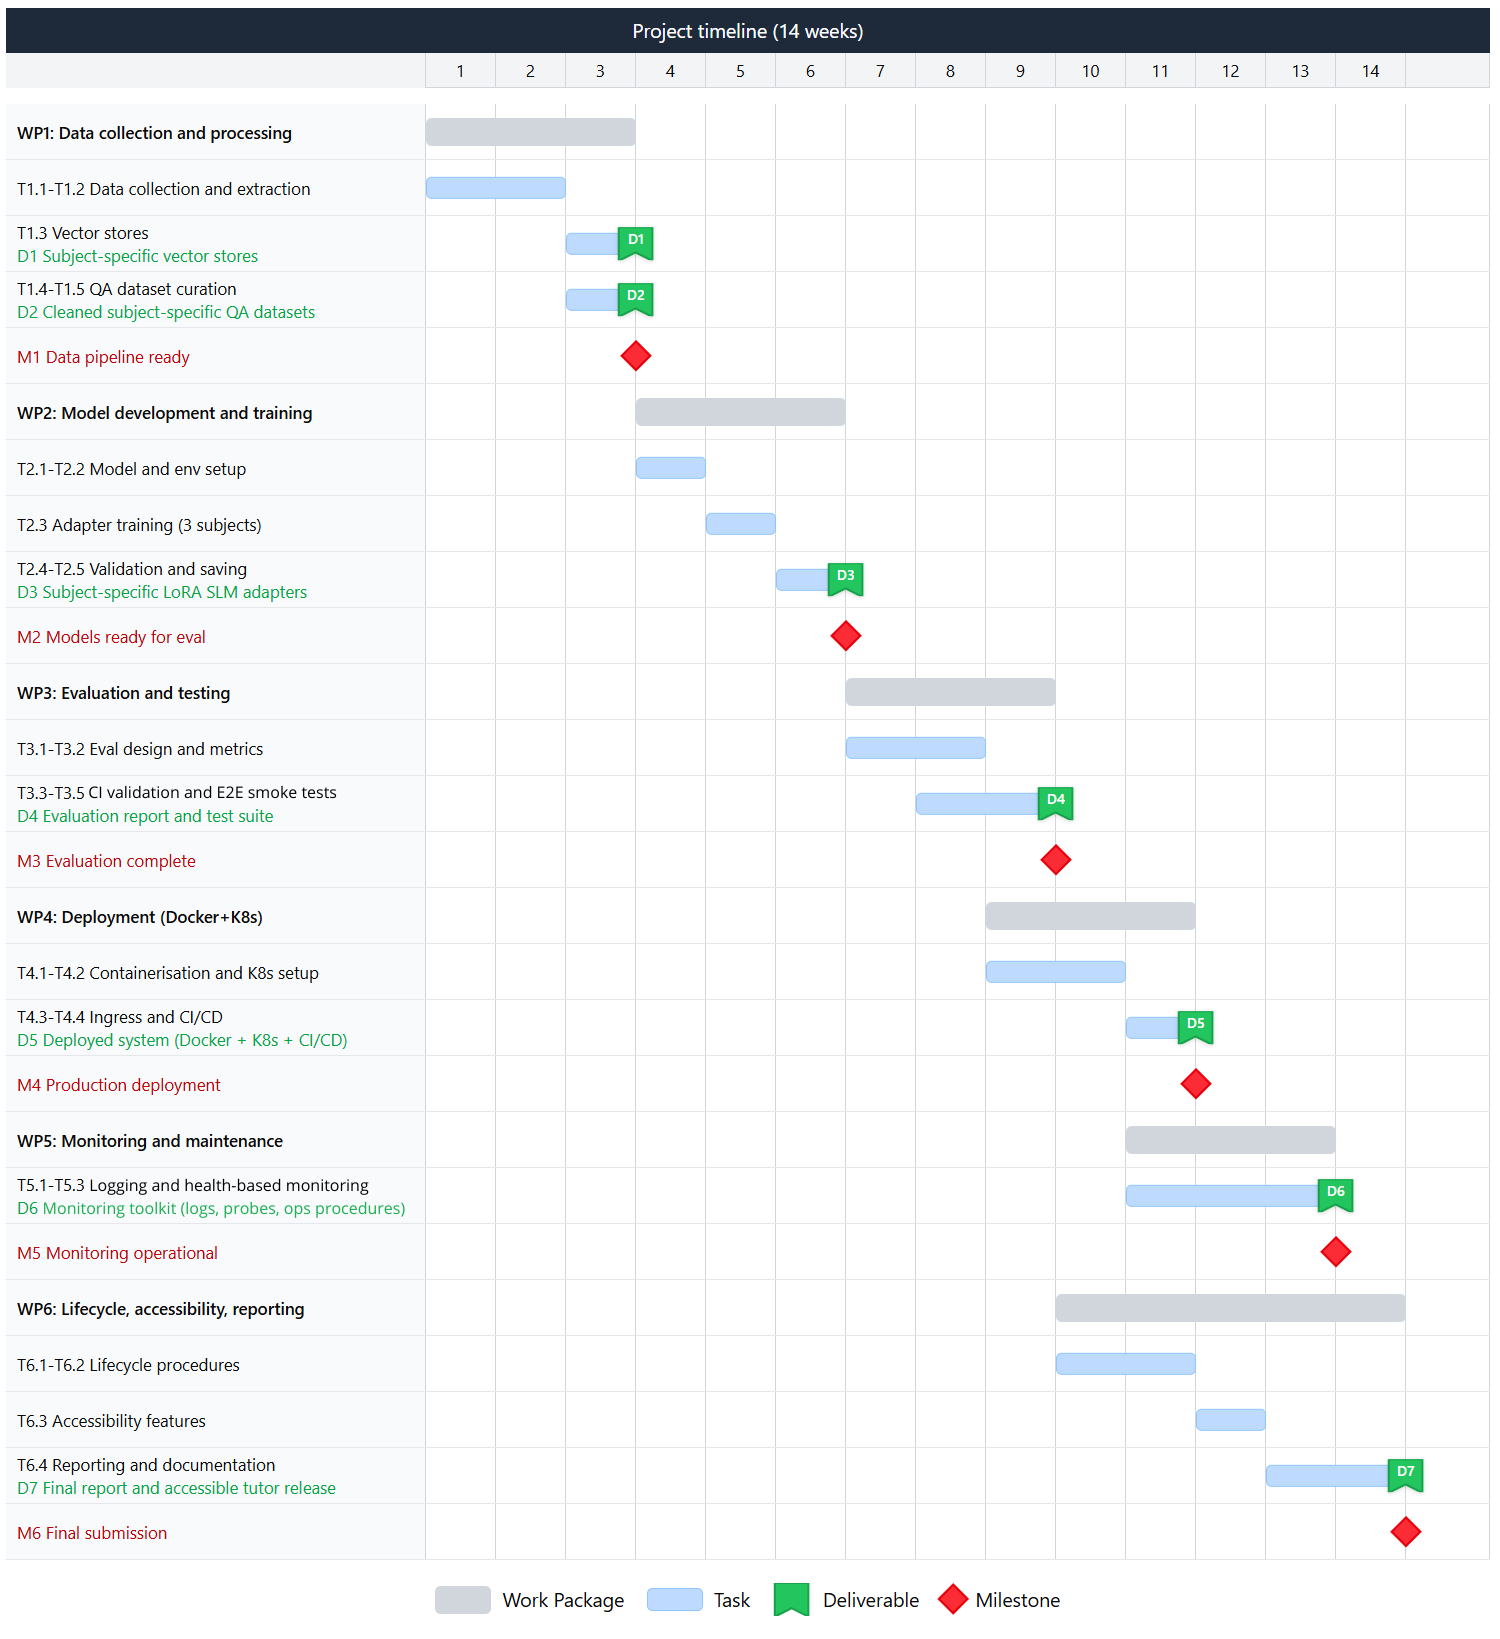
\includegraphics[width=\textwidth]{figs/gantt.png}
    \caption{Project timeline (14 weeks) with work packages (WP1-WP6), tasks, deliverables (D1-D7) and milestones (M1-M6).}
    \label{fig:project-timeline}
\end{figure}
\FloatBarrier

\subsection{WP1 - Data collection and processing}
The project begins with assembling the learning materials for the three subjects. The data consists of lecture presentations and tutorial sheets provided by the teaching team. These materials are usually distributed as PDF, PPTX, or DOCX files, depending on the module. All files are collected from the official module resources to ensure accuracy and relevance (Task T1.1).

The RAG pipeline does not require heavy preprocessing of the documents. Instead, each file is processed page by page, and a text representation is generated for each slide or section while keeping the original page index (Task T1.2). This makes it possible to link every retrieved chunk back to its specific slide or tutorial page.

Each page is then embedded and added to a subject-specific vector store (Task T1.3). Since the documents remain in their original format, the system can reference the exact page number or slide number when answering a question. This supports transparency and helps students verify the information. The resulting subject-specific vector stores constitute Deliverable D1.

Fine-tuning requires structured question-answer pairs, which are not directly present in lecture slides or tutorials. For each core concept or topic, an appropriate student-oriented question is formulated. The answer is then written in full sentences using the information from the slide or tutorial page (Task T1.4). This step ensures both accuracy and alignment with the real curriculum.

To increase efficiency, a semi-automatic pipeline supports this process. A script extracts text from each slide or tutorial page and identifies potential headings or keywords. These prompts generate candidate questions, which are then edited and improved by the researcher. The final datasets therefore combine automated support with careful human revision (Task T1.5). The curated QA datasets produced in this way form Deliverable D2 and are kept separate from the documents used for retrieval.

These datasets are separate from the files used for retrieval. While RAG preserves the complete structure of the original documents, fine-tuning is performed only on the curated question-answer pairs that follow a pedagogically meaningful format.

The processed pages and the curated question-answer datasets produced in this stage form the inputs for the training phase described next.

Taken together, Tasks T1.1-T1.5 deliver D1 (subject-specific vector stores) and D2 (curated QA datasets for each subject). Reaching this point for all three subjects defines milestone M1, at which the data pipeline is ready to support subsequent model training and evaluation.

\subsection{WP2 - Model Development and Training}
This stage uses the fine-tuning datasets constructed in the previous stage. The base model, Phi-4-mini-instruct, is loaded and configured to follow its official chat format (Task T2.1). LoRA is employed to perform parameter-efficient fine-tuning on Google Colab using a GPU runtime (Task T2.2). Each subject is trained independently using its own curated dataset (Task T2.3). This results in three lightweight LoRA adapters, one per subject, which can later be loaded alongside the base model inside each microservice.

During this stage, the behaviour of the base model is first validated to ensure that it loads correctly and fits into memory(Task T2.4). After fine-tuning, the trained adapters are saved and stored alongside configuration files that record the training parameters (Task T2.5). The output of this stage consists of three subject-specific SLM variants that can generate clearer, more accurate, and more context-aware answers than the base model alone. These three adapters together constitute Deliverable D3.

Taken together, Tasks T2.1-T2.5 produce D3, a set of subject-specific LoRA-based SLM adapters that can be loaded on top of the base model. Completion of these activities for all three subjects constitutes milestone M2, at which point the models are ready for systematic evaluation and comparison with the base model (Milestone M2).

\subsection{WP3 - Model Evaluation and Testing}

Once all three models have been trained, they are evaluated individually and then tested in the microservice setup. This stage evaluates the models from the previous stage and verifies their integration with the RAG components created earlier. Evaluation is performed both with and without RAG so that the contribution of fine-tuning can be measured separately from the contribution of retrieval (Task T3.1). The evaluation sets are used to assess correctness, clarity, and relevance, and automatic metrics such as BLEU-2, ROUGE-L, METEOR, and BERTScore F1 are computed (Task T3.2).

Technical validation is then performed to ensure that the deployed system behaves as expected. Component-level and service-level checks are covered through automated CI validation, including Python syntax checks, Kubernetes manifest validation, and security scans (Tasks T3.3-T3.4). End-to-end frontend smoke tests with Playwright validate the complete user flow from question submission to rendered response and sources (Task T3.5). The outcomes of this stage confirm deployment readiness and provide evidence of the impact of fine-tuning and RAG on answer quality.

The results of the quantitative and qualitative evaluation, together with the implemented automated CI checks and frontend end-to-end smoke tests, form Deliverable D4. An evaluation report and a verified test suite covering the core components of the system. Completion of Tasks T3.1-T3.5 and delivery of D4 constitute milestone M3, which marks the end of the evaluation phase and confirms that the system is ready to be deployed in a production-like environment (Milestone M3).


\subsection{WP4 - Deployment with Docker and Kubernetes}
This stage uses the validated models and the tested retrieval components to build the final system. Each subject-specific backend service is packaged into a Docker container that includes its FastAPI application and the corresponding fine-tuned adapter (Task T4.1). Subject-specific ChromaDB vector stores are deployed as separate services. Kubernetes is then used to orchestrate the services and provide stable routing, scaling, and fault isolation (Task T4.2).

An ingress controller routes external traffic to the correct subject service based on the URL path (Task T4.3). Continuous integration and delivery pipelines are created using GitHub Actions and Argo CD (Task T4.4). The output of this stage is a production-ready multi-service system that can be accessed consistently and maintained over time.

The deployed system, together with its Docker images, Kubernetes manifests, and CI/CD pipelines, forms Deliverable D5. Achieving a stable deployment of all three subject-specific services in the target environment, accessible behind a unified endpoint and updated automatically through CI/CD, defines milestone M4, the completion of the production deployment (Milestone M4).

\subsection{WP5 - Monitoring and Maintenance}
Once the three subject-specific microservices are deployed, the system must be observed continuously to ensure that it remains stable, responsive, and reliable. Monitoring focuses on the behaviour of the system in real time. This includes tracking request latency, error rates, model inference time, and the performance of the vector stores (Task T5.1). Each service exposes health check endpoints that allow Kubernetes to detect when a container becomes unresponsive and automatically restart it if necessary (Task T5.2).

To support operational observation, the system collects structured backend logs that describe startup behaviour, retrieval activity, and per-request inference latency. Health probes and container status provide an additional runtime signal in Kubernetes (Task T5.3). External observability tooling such as Prometheus and Grafana is identified as future work rather than part of the implemented stack.

Maintenance activities are performed in response to the insights gained from monitoring. For example, if a model becomes slow under higher demand, its resources can be adjusted or replicas can be scaled up within Kubernetes. If retrieval quality decreases due to new teaching materials, the vector store can be refreshed. Maintenance therefore ensures that the deployed tutor remains functional and stable as a live service, addressing operational concerns rather than long-term development.

The output of this stage is a system that not only runs in production but remains actively supervised and supported, reducing downtime and improving reliability for its users.

The combination of monitoring configuration, structured logging, health checks, and documented operational procedures constitutes Deliverable D6, the monitoring and maintenance toolkit. When these elements are in place and routinely used to guide maintenance and scaling decisions, milestone M5 is reached, indicating that monitoring is fully operational (Deliverable D6, Milestone M5).

\subsection{WP6 - Lifecycle Management, Accessibility, and Reporting}

While monitoring focuses on short-term system behaviour, lifecycle management addresses the long-term evolution of the Agentic AI Tutor. Because course materials change over time, the system must support the integration of new lectures and tutorials without being rebuilt from scratch. Version control ensures that older models, datasets, and configurations remain accessible, allowing experiments and deployments to be repeated reliably (Task T6.1).

Lifecycle management also includes planning for future fine-tuning or retraining. When a module's content changes significantly, a new fine-tuning dataset may be required, followed by the creation of an updated LoRA adapter. In such cases, the entire pipeline can be executed again using the same structured process, ensuring consistency between iterations of the tutor service (Task T6.2).

Accessibility is an essential part of this stage because the tutor is intended for a diverse group of learners. Features such as text-to-speech output, optional talking-head avatar rendering, and interface adjustments are addressed during this phase (Task T6.3), while speech-based input is treated as future work.

Finally, this stage includes the preparation of documentation and reporting. The dissertation chapters describing implementation, evaluation, limitations, and future work are written during this phase (Task T6.4). As a result, lifecycle management connects the technical development of the system with its long-term sustainability, user accessibility, and academic reporting requirements.

Together, these activities produce Deliverable D7. A final report and accessible release of the tutor, including documentation and the implemented accessibility features. Completion of Tasks T6.1-T6.4 and delivery of D7 constitutes milestone M6, which coincides with the final submission of the dissertation and the end of the first full lifecycle of the system (Deliverable D7, Milestone M6).

The remainder of this dissertation is organised as follows.
Chapter~\ref{chap:literature_review} reviews the theoretical foundation of the project, including transformer models, Small Language Models, their applications in education, and the challenges they address such as hallucinations, cost, and accessibility.
Chapter~\ref{chap:technical_review} presents the technical choices behind the system, evaluating candidate SLMs, selecting fine-tuning methods, and outlining the supporting MLOps infrastructure (containerisation, CI/CD, and orchestration).
Chapter~\ref{chap:methodology} explains the methodological decisions, comparing knowledge-integration techniques (fine-tuning, RAG, CAG) and justifying the selection of RAG and MLOps as the core workflow.
Finally, Chapter~\ref{chap:implementation} describes the practical development process following the MLOps lifecycle, including data preparation, fine-tuning, evaluation, deployment with Docker and Kubernetes, monitoring, and long-term lifecycle management.
